\documentclass[12pt,openright,oneside,a4paper,brazil]{abntex2}
\usepackage[utf8]{inputenc}
\counterwithout{section}{section}
\counterwithout{figure}{chapter}
\counterwithout{table}{chapter}
\setlength{\parindent}{1.3cm}
\usepackage{indentfirst}
\setlength{\parskip}{0.2cm}
\usepackage[bottom=2cm,top=3cm,left=3cm,right=2cm]{geometry}
\usepackage{graphicx}
\graphicspath{{figuras/}}
\usepackage{placeins}
\usepackage{cite}
\usepackage{url}
\usepackage{breakurl}
\include{bibliografia}

\makeatletter
\setlength{\@fptop}{0pt}
\makeatother

\begin{document}

\textual
\begin{center}
 {\large Anemômetroultrassônico}\\[0.2cm]
 \end{center}
 
Existem vários tipos de anemômetros, mas entre eles o mais vantajoso por ter uma rápida resposta, boa exatidão nos dados e é possível ser implementado em ambientes com extremas temperaturas e pressão é o ultrassónico. Este sensor basicamente utiliza o som que é desencadeado pelo movimento das partículas que o compõe, estimando assim a velocidade do vento. 

O processo de recolhimento dos dados de velocidade e direção do vento é o seguinte,primeiramente com o sinal de excitação, transmite-o para um transistor-transmissor que posteriormente repassa para um transistor-transmissor um sinal ultrassônico, neste processo de transição o sinal sofre alterações, desse modo no transistor-transmissor o sinal é processado e analisado para entregar as informações requeridas. O arranjo do equipamento é essencial para o recolhimento dos dados, por causa de seu formato, que contémum tetraedro com três transdutores em cada extremidade, sendo possível detectar a direção do vento e assim sua velocidade. 

Abaixo especificações técnicas de um anemômetro ultrassônico (Vaisala WINDCAP® WMT700):

{\large Velocidade do vento}\\
Faixa de medição	- 

701	0...40 m/s

702	0...65 m/s

703	0...75 m/s

Precisão	-	+/- 0,2 m/s ou 3 \% da leitura, o que for maior

Limite inicial - 0,01 m/s

Resolução - 0,01 m/s\\

{\large Direção do vento}

Faixa de medição - 0 ... $300\,^{\circ}\mathrm{C}$

Precisão - +/- $2\,^{\circ}\mathrm{C}$

Limite inicial - 0,1 m/s

Resolução - $1\,^{\circ}\mathrm{C}$,

{\large Saídas}

Taxa de transmissão - 300, 1200, 2400, 4800, 9600, 19200, 38400, 57600, 115200

Médias disponíveis -  máx. 3600 s

Intervalo de atualização de leitura - máx. 4 Hz

Unidades

Saídas digitais - m/s, nós, mph, km/h

Saídas analógicas - V, mA, Hz

Temperatura virtual - graus Celsius

{\large Geral}

Temperatura de operação	- -10 ... +60 ou -40 ... +60 ou -55 ... $+70\,^{\circ}\mathrm{C}$,
\newpage

\begin{center}
 {\large Sensor de pH}\\[0.2cm]
 \end{center}
 
{\large Especificação do sensor de pH}\\
 O sensor de pH da água é de extrema importância para o projeto da “planta de abastecimento de água potável através da umidade do ar” pois monitora um dos índices de qualidade da água especificados pela ANA(agência nacional de águas). 
 
	Para aplicações industriais, o método de medição de pH mais empregado é o eletrodo de vidro(Solé, 1979).Os eletrodos de pHpossuem basicamente o mesmo funcionamento que as baterias: transferem uma tensão mínima que poderá ser detectada por um medidor ou um regulador de pH. A diferençaé que os eletrodos de pH não produzem tensão de forma contínua, a não ser quando são introduzidos num líquido

{\large Calibração de sensores de pH}\\
O período de calibração de um sensor de pH depende do contexto em que o sensor será aplicado e do tipo de sensor que será utilizado. O tipo de sensor a ser utilizado pode variar de acordo com parâmetros como temperatura. O sensor de pH pode vir acoplado a um sensor de condutividade, entre outros. Apesar de existirem vários tipos, todo eletrodo de pH requer calibração periódica. Uma calibração em dois pontos caracteriza um eletrodo com um medidor de pH específico.

{\large Sensor ORP}\\
O sensor ORP é similar ao sensor pH quanto ao seu funcionamento, porém, ao invés de seu eletrodo ser envolvido por vidro, é geralmente envolvido por platina ou ouro, devido ao fato de esses metais não interferirem nas reações químicas. Nos sensores ORP, o gel interno recebe a corrente elétrica provinda do meio e a transmite ao interior do sensor. Posteriormente, o fio e prata pura transmite a corrente positiva ao para o cabo de conexão, que leva o sinal recebido ao controlador.
\newpage

\begin{center}
 {\large Métodos de Processamento de Sinais}\\
 \end{center}
 O processamento de sinais será realizado por meio de um sistema de sensoriamento do local onde se encontrará a planta de abastecimento. Os sensores farão a varredura do local, coletando dados sobre a qualidade da água já tratada provinda da umidade do ar. Os dados a serem coletados estão de acordo com o Índice de Qualidade da Água(IQA). Para cada fator a ser monitorado de acordo com o IQA existirá um sensor relacionado. 
 
	Como foi dito anteriormente, almeja-se utilizar a sonda YSI EXO, que coleta dados de 6 sensores substituíveis e que estão de acordo com o Índice de Qualidade da Água(IQA). A sonda YSI EXO é comandada por um software embarcado. Além disso, a própria sonda, além de possuir um sistema de sensoriamento, processa suas próprias informações, enviando-as à uma central computadorizada.
\newpage
\begin{center}
 {\large Especificações do Sensor de Umidade Relativa e Temperatura do Ar}\\
 \end{center}
{\large Características:}\\
 \begin{itemize}
\item Processamento digital de sinal
\item Umidade relativa e temperatura do ar em um único sensor
\item Alta acurácia de leitura e linearização
\item Sinais de saída condicionados
\item Excelente estabilidade de longo termo
\item Baixo tempo de resposta
\item 100 \% intercambialidade
 \end{itemize}
{\large Construção:}\\
O invólucro do sensor e do circuito eletrônico é moldado em plástico injetado e estabilizado para U.V. O invólucro do circuito é selado, sendo à prova de respingos e poeira. Todas as conexões elétricas são feitas através de um conector selado na base do sensor. O sensor opera de 0 a 100\% umidade relativa. Os transdutores internos não sofrem danos mesmo com condensação. O circuito digital do sensor realiza a compensação de temperatura e a linearização do sinal de saída. O armazenamento dos dados de calibração do sensor em memória interna não volátil fornece uma maior acurácia nas leituras.
\begin{figure}
\centering
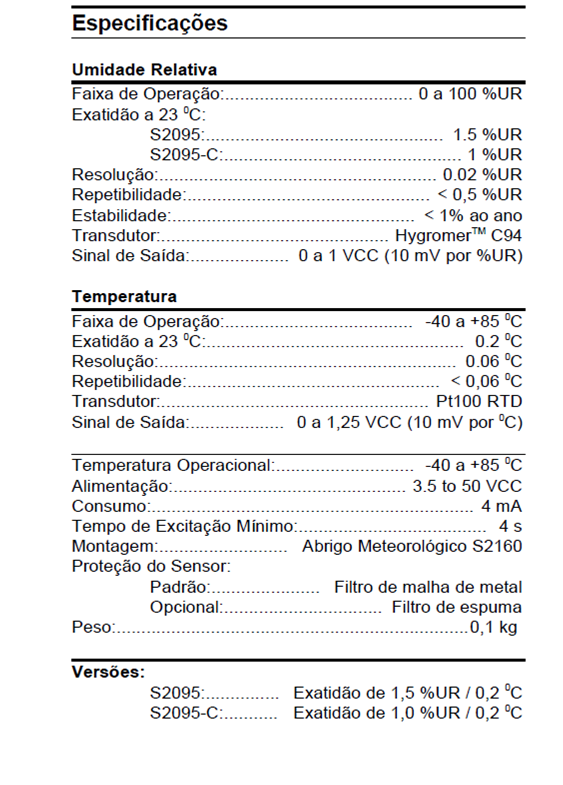
\includegraphics[scale=1]{umidade}
\end{figure}
\FloatBarrier
\newpage
\begin{center}
 {\large Sensores de Processamento de Sinais para Umidade do Ar}\\
 \end{center}
 O uso de equipamentos que usa o processamento de sinais é de suma importância para extrair informações do clima para a aplicação de retirada de água a partir da umidade do ar. O uso de um sensor de umidade relativa e temperatura do ar combinam sensores de umidade e temperatura de alta precisão em um único instrumento. Ambos os sensores fornecem sinais de saída diretamente proporcionais à umidade relativa e temperatura. O  processamento digital de sinais embutido no sensor garante uma precisa linearização dos sinais de saída em toda a faixa de operação e total intercambialidade do sensor. 
 
Operação: Para melhor desempenho, ele deve ser posicionado em local com boa circulação de ar e longe de grandes construções, como  edifícios ou muros. A membrana protetora do sensor de umidade relativa deve ser regularmente limpa. Sempre que possível, a limpeza deve ser feita sem a remoção do filtro. Em aplicações que envolvem contínuo contato com água ou poeira grossa, um filtro de espuma  opcional esta disponível. A calibração do sensor de temperatura não é necessária. Para o sensor de umidade, a calibração pode ser feita a cada 6 a 12 meses para garantia de máximo desempenho.
 Características:
 \begin{itemize}
\item Processamento digital de sinal
\item Umidade relativa e temperatura do ar em um único sensor
\item Alta acurácia de leitura e linearização
\item Sinais de saída condicionados
\item Excelente estabilidade de longo termo
\item Baixo tempo de resposta
\item 100 \% intercambialidade
 \end{itemize}
 \newpage
\begin{center}
 {\large Parâmetros da qualidade da água}\\
 \end{center}
Existe um indicador chamado Índice de Qualidade das Águas (IQA), que é o principal índice de qualidade da água utilizado em todo o país. A finalidade do desenvolvimento de tal índice é analisar a qualidade da água após o tratamento da mesma.

Como desvantagens do uso do IQA, deve-se citar o fato de o índice não contemplar vários parâmetros importantes para o abastecimento público, tais como:
\begin{itemize}
\item Substâncias tóxicas (ex: metais pesados, pesticidas, compostos orgânicos);
\item Protozoários patogênicos
\item Substâncias que interferem nas propriedades organolépticas da água.

\end{itemize}

O IQA é composto por nove parâmetros, que têm seus respectivos pesos, os quais foram fixados de acordo com sua importância global na determinação da qualidade da água. Veja na tabela a seguir:
\begin{figure}[h]
\centering
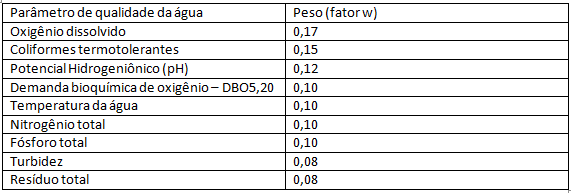
\includegraphics[scale=0.8]{tabela}
\end{figure}
\FloatBarrier
Além de seu peso (w), cada parâmetro possui um valor de qualidade (q), obtido do respectivo gráfico de qualidade em função de sua concentração ou medida. Observe a figura abaixo:
\begin{figure}[h]
\centering
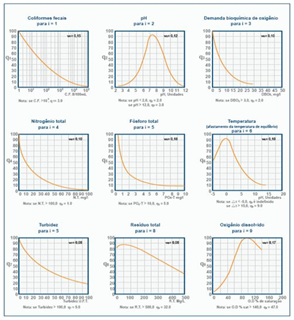
\includegraphics[scale=0.8]{grafico}
\end{figure}
\FloatBarrier

O cálculo do IQA é dado da seguinte forma:

\begin{figure}[h]
\centering
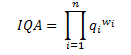
\includegraphics[scale=1]{eq1}
\end{figure}

Onde:
\begin{itemize}

\item IQA: Índice de Qualidade das Águas. Um número de 0 a 100;
\item qi: qualidade do i-ésimo parâmetro. Um número entre 0 e 100, obtido do respectivo gráfico de qualidade, em função de sua concentração ou medida (resultado da análise).
\item wi: peso correspondente ao i-ésimo parâmetro fixado em função da sua importância para a conformação global da qualidade, isto é,  um número de 0 a 1, de forma que:
\begin{figure}[h]
\centering
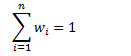
\includegraphics[scale=01]{eq2}
\end{figure}
\FloatBarrier
\end{itemize}

Sendo n o número de parâmetros que entram no cálculo do IQA.
A descrição dos parâmetros que compõe o IQA será efetuada a seguir.
\begin{itemize}
\item Oxigênio dissolvido (OD): é um fator limitante para a manutenção da vida aquática e de processos de autodepuração em sistemas aquáticos naturais e estações de tratamento de esgotos [2]. Águas limpas têm concentração de oxigênio, na maioria das vezes, maior ou igual a 5 mg/L. 
No que se refere aos processos que contribuem para a introdução do oxigênio na água, pode-se citar, além da fotossíntese, determinados processos físicos os quais dependem das características hidráulicas dos corpos d’água, por exemplo: velocidade da água.
\item Coliformes termotolerantes: São bactérias não patogênicas que ocorrem no trato intestinal de animais de sangue quente e são indicadoras de poluição da água causada pelos esgotos domésticos. Quando há grande quantidade dessas bactérias na água, há a possibilidade de existir microorganismos capazes de transmitir doenças de veiculação hídrica[1].
\item Potencial Hidrogeniônico (pH): O pH (medida que determina a acidez ou basicidade de uma mistura) é capaz de alterar o metabolismo de diversas espécies aquáticas.Dessa forma, o CONAMA estabelece que o pH deve estar entre 6 e 9 para a proteção da vida aquática.
\item Demanda Bioquímica de Oxigênio (DBO5,20): representa a quantidade necessária de oxigênio para oxidar a matéria orgânica aquática por meio da decomposição microbiana aeróbia. A ocorrência de altos valores de DBO5,20 acarreta na diminuição   dos valores de oxigênio dissolvido (OD). A sigla DBO5,20 equivale à quantidade de oxigênio consumido em 5 dias a uma temperatura de 20C.
\item Temperatura da água: influencia em diversos parâmetros físico-químicos da água (ex: tensão superficial e a viscosidade) além de afetar o crescimento e reprodução de espécies aquáticas.
\item Nitrogênio total: O nitrogênio pode ocorrer nos corpos d’água em diversas formas (orgânica, amoniacal, nitrito e nitrato). Os nitratos são tóxicos aos humanos.
Além disso, como os compostos de nitrogênio nutrem os processos biológicos, a grande concentração de nitrogênio (juntamente com outros nutrientes) em corpos d’água causa a eutrofização, que prejudica o abastecimento público e a preservação da vida aquática. A principal fonte de nitrogênio em corpos d’água é o lançamento de esgotos sanitários e efluentes industriais.Em áreas agrícolas, o escoamento da água das chuvas em solos que receberam fertilizantes também é uma fonte de nitrogênio, assim como a drenagem de águas pluviais em áreas urbanas[1].
\item Fósforo total: Assim como o nitrogênio, o fósforo (em excesso) causa a eutrofização das águas. As principais fontes de fósforo são os esgotos domésticos, pelo fato de eles terem a presença de detergentes superfostadados e das próprias fezes. Além disso, a drenagem pluvial de áreas agrícolas e urbanas também é uma fonte significativa. Entre os efluentes industriais destacam-se os das indústrias de fertilizantes, alimentícias, laticínios, frigoríficos e abatedouros [1].
\item Turbidez: indica o grau de atenuação que um feixe de luz sofre ao atravessar a água. Tal atenuação é devida à absorção e espalhamento de luz causada pelos sólidos em suspensão. A principal fonte de turbidez é a erosão dos solos (chuvas trazem os corpos sólidos).
\item Resíduo total: é a matéria a qual permanece após a evaporação, secagem ou calcinação da amostra de água durante um determinado tempo e temperatura.

\end{itemize}
Existe uma empresa chamada Clean Environment Brasil, que fornece equipamentos de monitoramento e controle da água à ANA (Agência Nacional de Águas). Eles produzem várias sondas multiparamétricas (conseguem monitorar vários parâmetros em uma só sonda). 
Seria interessante utilizar a sonda YSI EXO, que coleta dados de 6 sensores substituíveis, pois ela também é usada pela ANA para determinar a qualidade da água.

As opções de sensores para esse tipo de sonda são:
\begin{itemize}
\item Condutividade e temperatura;
\item Oxigênio dissolvido;
\item Matéria Orgânica Dissolvida (fluorescência);
\item pH ou pH/ORP;
\item Profundidade (que já é integrado);
\item Algas totais (canal duplo para clorofila e algas azuis/verdes);
\item Turbidez [3].
\end{itemize}
Assim, com apenas um equipamento relativamente leve (3,6 kg com baterias e sensores instalados) de pequenas dimensões ($\Phi$ = 7,62cm e comprimento = 71,10cm) é possível monitorar a maioria dos parâmetros do índice IQA.
\newpage
Referências

[1] - http://portalpnqa.ana.gov.br/indicadores-indice-aguas.aspx

[2] - http://www.cetesb.sp.gov.br/mortandade/causas\_oxigenio.php

[3] - http://www.clean.com.br/site/ysi-exo-2/

[4] - http://www.inicepg.univap.br/cd/INIC\_2006/inic/inic/07/INIC0000904.ok.pdf

[5] - http://br.vaisala.com/br/products/windsensors/Pages/WMT700.aspx

\end{document}